\documentclass[tikz, border=10pt]{standalone}
\usepackage{helvet}
\renewcommand{\familydefault}{\sfdefault}
\usepackage{tikz}
\usetikzlibrary{arrows.meta, positioning, fit, calc, shapes.geometric, decorations.pathreplacing}

\definecolor{emeraldpine}{HTML}{1A4D3E}
\definecolor{harvardcrimson}{HTML}{A51C30}
\definecolor{ethdarkblue}{HTML}{1F407A}
\definecolor{ethpetrol}{HTML}{007A87}
\definecolor{ethbronze}{HTML}{B87333}
\definecolor{ethpurple}{HTML}{5B4B8A}
\definecolor{ink}{HTML}{1A202C}
\definecolor{softink}{HTML}{4A5568}
\definecolor{paleink}{HTML}{A0AEC0}
\definecolor{cardbg}{HTML}{F8FAFC}
\definecolor{shadecolor}{HTML}{F4F6F9}

\begin{document}
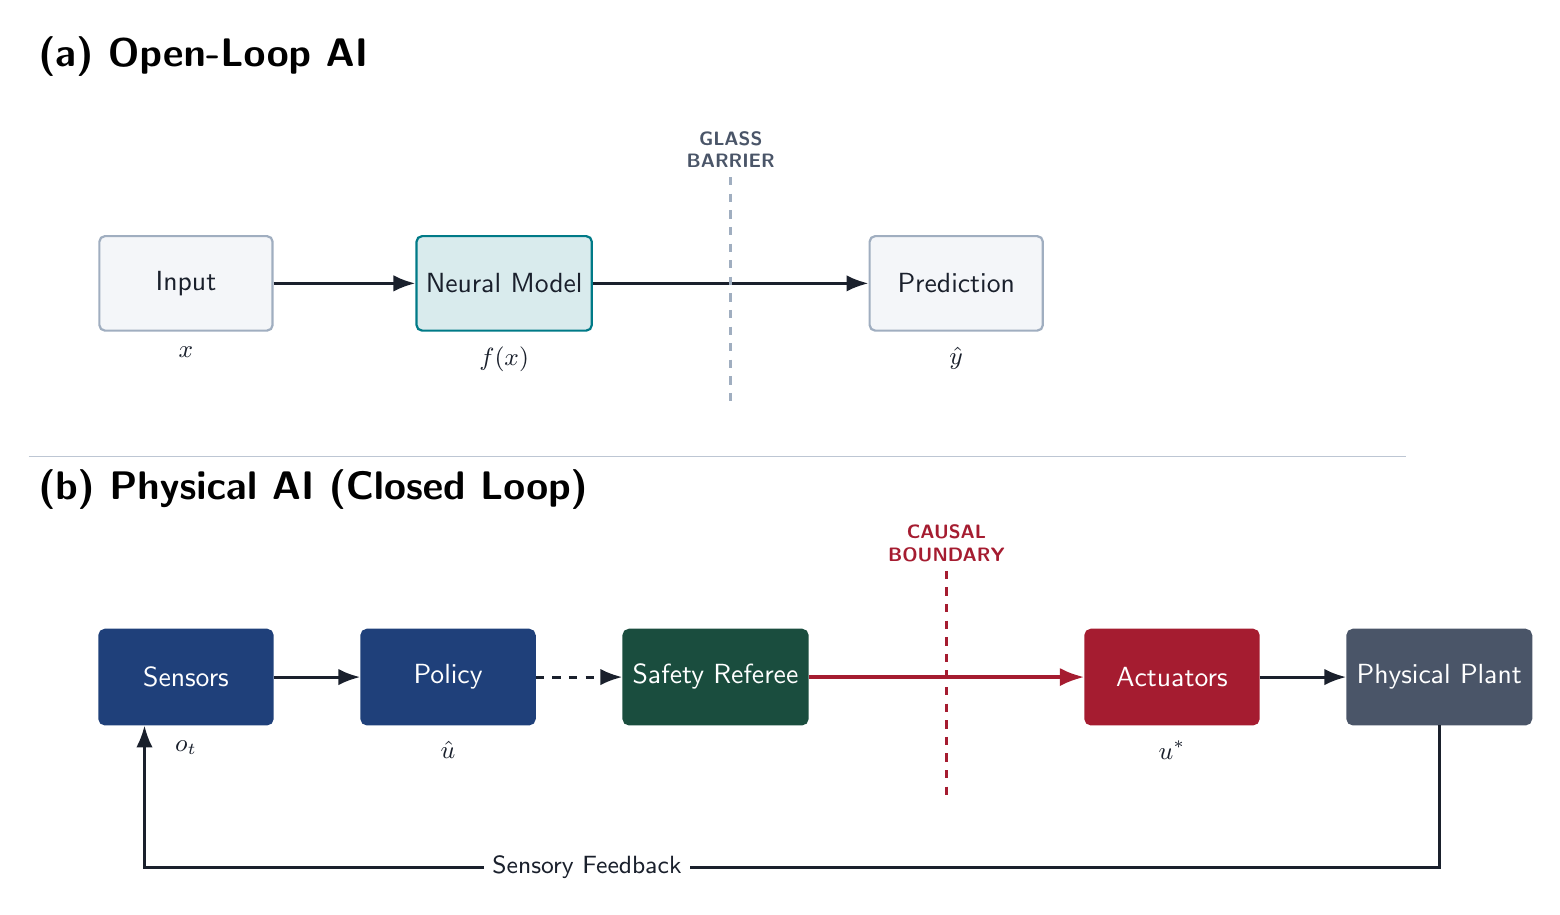
\begin{tikzpicture}[
    >=Latex,
    node distance=1.5cm,
    font=\sffamily,
    box/.style={
        draw, rounded corners=2pt, minimum height=1.2cm, minimum width=2.2cm, align=center, thick
    },
    panelLabel/.style={
        font=\sffamily\bfseries\Large, anchor=south west
    },
    arr/.style={->, line width=1.1pt, ink},
    darr/.style={->, dashed, line width=1.1pt, ink},
    barline/.style={dashed, line width=1.2pt, paleink}
]

% Panel (a)
\node[panelLabel] (pA) at (-1, 3.5) {(a) Open-Loop AI};

\node[box, fill=shadecolor, draw=paleink, text=ink] (input) at (1, 1) {Input};
\node[anchor=north, font=\sffamily\small, text=ink, yshift=-2pt] at (input.south) {$x$};

\node[box, fill=ethpetrol!15, draw=ethpetrol, text=ink, right=1.8cm of input] (model) {Neural Model};
\node[anchor=north, font=\sffamily\small, text=ink, yshift=-2pt] at (model.south) {$f(x)$};

\node[box, fill=shadecolor, draw=paleink, text=ink, right=3.5cm of model] (pred) {Prediction};
\node[anchor=north, font=\sffamily\small, text=ink, yshift=-2pt] at (pred.south) {$\hat{y}$};

\draw[arr] (input) -- (model);
\draw[arr] (model) -- (pred);

% Vertical Glass Barrier line with clean header
\coordinate (gbMid) at ($(model.east)!0.5!(pred.west)$);
\node[font=\sffamily\bfseries\scriptsize, text=softink, align=center] (gbLabel) at (gbMid |- 0, 2.7) {GLASS\\BARRIER};
\draw[barline] (gbLabel.south) -- (gbMid |- 0, -0.6);

% Divider
\draw[draw=paleink!70, line width=0.6pt] (-1, -1.2) -- (16.5, -1.2);

% Panel (b)
\node[panelLabel] (pB) at (-1, -2.0) {(b) Physical AI (Closed Loop)};

\node[box, fill=ethdarkblue, draw=ethdarkblue, text=white] (sensors) at (1, -4.0) {Sensors};
\node[anchor=north, font=\sffamily\small, text=ink, yshift=-2pt] at (sensors.south) {$o_t$};

\node[box, fill=ethdarkblue, draw=ethdarkblue, text=white, right=1.1cm of sensors] (policy) {Policy};
\node[anchor=north, font=\sffamily\small, text=ink, yshift=-2pt] at (policy.south) {$\hat{u}$};

\node[box, fill=emeraldpine, draw=emeraldpine, text=white, right=1.1cm of policy] (safety) {Safety Referee};

\node[box, fill=harvardcrimson, draw=harvardcrimson, text=white, right=3.5cm of safety] (actuators) {Actuators};
\node[anchor=north, font=\sffamily\small, text=ink, yshift=-2pt] at (actuators.south) {$u^*$};

\node[box, fill=softink, draw=softink, text=white, right=1.1cm of actuators] (plant) {Physical Plant};

\draw[arr] (sensors) -- (policy);
\draw[darr] (policy) -- (safety);
\draw[arr, draw=harvardcrimson, line width=1.3pt] (safety) -- (actuators);
\draw[arr] (actuators) -- (plant);

% Causal Boundary with clean header
\coordinate (cbMid) at ($(safety.east)!0.5!(actuators.west)$);
\node[font=\sffamily\bfseries\scriptsize, text=harvardcrimson, align=center] (cbLabel) at (cbMid |- 0, -2.3) {CAUSAL\\BOUNDARY};
\draw[dashed, line width=1.2pt, harvardcrimson] (cbLabel.south) -- (cbMid |- 0, -5.6);

% Feedback loop with generous clearance
\draw[arr] (plant.south) -- ++(0,-1.8) -| ([xshift=-15pt]sensors.south);
\node[font=\sffamily\small, text=ink, fill=white, inner sep=3pt, rounded corners=2pt] 
    at ($(sensors.south)!0.32!(plant.south) + (0, -1.8)$) {Sensory Feedback};

\end{tikzpicture}
\end{document}
